\section{Energy Production}

While the transport of nutrients is required to build new cell mass, the
metabolic pathways involved in assimilation both consumes and generates energy
in the form of NTPs. The high-energy phosophodiester bonds of (primarily) ATP
power a variety of cellular processes that drive biological systems away
from thermodynamic equilibrium. Our next class of estimates consider the energy budget
of a dividing cell in terms of the synthesis of ATP from ADP and inorganic
phosphate as well as maintenance of the electrochemical proton gradient which powers it.

\subsection{ATP Synthesis}

Hydrolysis of the terminal phosphodiester bond of ATP forming ADP and an
inorganic phosphate is a kinetic driving force in a wide array of biochemical
reactions. One such reaction is the formation of peptide bonds during
translation which requires $\approx$ 2 ATPs for the charging of an amino acid
to the tRNA and $\approx$ 2 ATP equivalents for the formation of the peptide
bond between amino acids. Together, these energetic costs consume $\approx$
80\% of the cells ATP budget (BNID: 107782; 106158; 101637; 111918,
\cite{milo2010}). The pool of ATP is produced by the F$_1$-F$_O$ ATP synthase
-- a membrane-bound rotary motor which under ideal conditions can yield
$\approx$ 300 ATP per second (BNID: 114701; \cite{milo2010, weber2003}).

To estimate the total number of ATP equivalents consumed during a cell cycle, we
will make the approximation that there are $\approx 3\times10^6$ proteins per
cell with an average protein length of $\approx$ 300 peptide bonds (BNID:
115702; 108986; 104877, \cite{milo2010}). Together, we
arrive at the estimate that the typical \textit{E. coli} cell consumes $\approx
5 \times 10^9$ ATP per cell cycle on protein synthesis alone and $\approx
6\times 10^9$ ATP in total. Assuming that the ATP synthases are operating at
their fastest possible rate, we arrive at an estimate that $\approx$ 3000  ATP
synthases are needed to keep up with the energy demands of the cell. This
estimate and a comparison with the data are shown in \FIG{energy_production}(A).
Despite our assumption of maximal ATP production rate per synthase and
approximation of all NTP consuming reactions being the same as ATP, we find that
an estimate of a few thousand complete synthases per cell to agree well with the
experimental data.

\subsection{Generating the Proton Electrochemical Gradient}
In order to produce ATP, the F$_1$-F$_O$ ATP synthase itself must consume
energy. Rather than burning through its own product, this intricate
macromolecular machine has evolved to exploit the electrochemical potential
established across the inner membrane through cellular respiration. This
electrochemical gradient is manifest  by the pumping of protons into the
intermembrane space via the electron transport chains as they reduce NADH. In
\textit{E. coli}, this potential difference is $\approx -$200 mV (BNID: 102120,
\cite{milo2010}). As estimated in the supporting information, this potential
difference is generated by maintaining $\approx 2\times 10^4$ protons in the
intermembrane space.

However, the constant rotation of the ATP synthases would rapidly abolish
this potential difference if it were not being actively maintained. To
undergo a complete rotation (and produce a single ATP), the F$_1$-F$_O$ ATP
synthase must shuttle $\approx$ 4 protons across the membrane into the
cytosol (BNID: 103390, \cite{milo2010}). With $\approx$ 3000 ATP synthases each
generating 300 ATP per second, the $2 \times 10^4$ protons establishing the 200
mV potential would consumed in only a few milliseconds! This brings us
to our next estimate: how many electron transport complexes are needed to
support the consumption rate of the ATP synthases?

The electrochemistry of the electron transport complexes of \textit{E. coli}
have been the subject of intense biochemical and biophysical study over the past
half century \citep{ingledew1984, khademian2017,cox1970,henkel2014}. A recent
work \citep{szenk2017} examined the respiratory capacity of the \textit{E. coli}
electron transport complexes using structural and biochemical data, revealing
that each electron transport chain rapidly pumps protons into the intermembrane
space at a clip of $\approx$ 5000 protons per second (BIND: 114704; 114687,
\cite{milo2010}). Using our estimate of the number of ATP synthases required per
cell (\FIG{energy_production}(A)), coupled with these recent measurements, we
estimate that $\approx 1000$ electron transport complexes would be necessary to
facilitate the $\approx 4\times 10^6$ protons per second diet of the celllular
ATP synthases. This estimate is in agreement with the number of complexes
identified in the proteomic datasets (plot in \FIG{energy_production}(B)).

% [GC: I think we really need to comment on the growth rate dependence here and
% see if we can make any sense of it with increasing surface area.]

\begin{figure}
    \begin{fullwidth}
        \centering{
            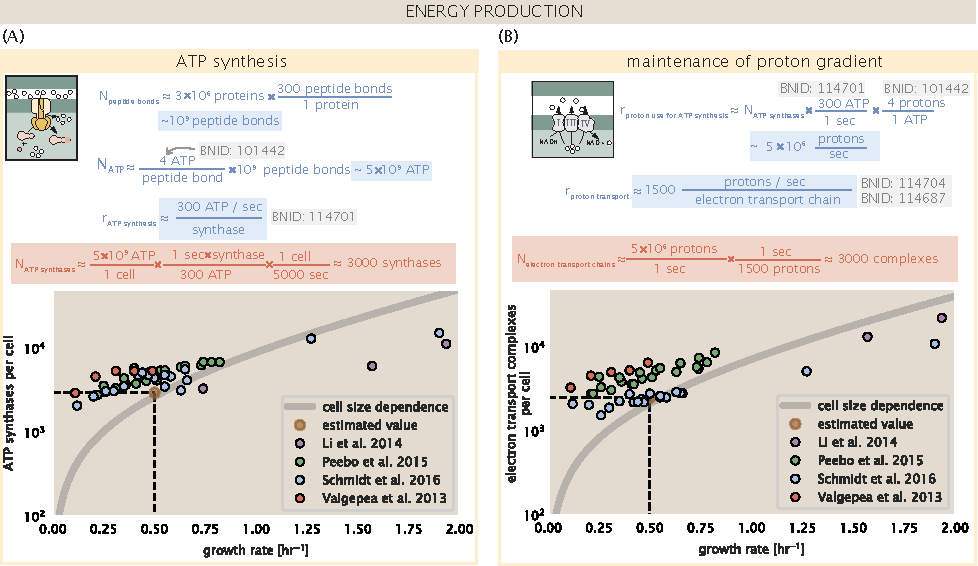
\includegraphics{main_figs/fig4_energy_production.pdf}
            \caption{\textbf{The abundance of F$_1$-F$_O$ ATP synthases and
            electron transport chain complexes as a function of growth
            rate.}(A) Estimate of the number of F$_1$-F$_O$ ATP synthase
            complexes needed accommodate peptide bond formation and other NTP
            dependent processes Points in plot at bottom correspond to the
            mean number of complete F$_1$-F$_O$ ATP synthase complexes that
            can be formed given proteomic measurements and the subunit
            stoichiometry
            [AtpE]$_{10}$[AtpF]$_2$[AtpB][AtpC][AtpH][AtpA]$_{3}$[AtpG][AtpD]$_3$.
            (B) Estimate of the number of electron transport chain complexes
            needed to maintain a membrane potential of $-$200 mV given
            estimate of number of F$_1$-F$_O$ ATP synthases from (A). Points
            in plot correspond to the average number of complexes identified
            as being involed in aerobic respiratoion by the Gene Ontology
            identifier GO:0019646 that could be formed given proteomic
            observations. These complexes include cytochromes \textit{bd1}
            ([CydA][CydB][CydX][CydH]), \textit{bdII} ([AppC][AppB]),
            \textit{bo$_3$},([CyoD][CyoA][CyoB][CyoC]) and NADH:quinone
            oxioreducase I
            ([NuoA][NuoH][NuoJ][NuoK][NuoL][NuoM][NuoN][NuoB][NuoC][NuoE][NuoF][NuoG][NuoI])
            and II ([Ndh]).}
        \label{fig:energy_production}
        }
    \end{fullwidth}
\end{figure}


\subsection{Energy production in a crowded membrane.}

For each protein considered so far, the data shows that in general their numbers
increase with growth rate. This is in part a consequence of the increase in cell
length and width at that is common to many rod-shaped bacteria at faster growth
rates \citep{ojkic2019, harris2018}. For the particular case of \textit{E.
coli}, the total cellular protein and cell size increase logarithmically with
growth rate \citep{schaechter1958, si2017}. Indeed, this is one reason why we
have considered only a single, common growth condition across all our estimates
so far. Such a scaling will require that the total number of proteins and net
demand on resources also grow in proportion to the increase in cell size divided
by the cell's doubling time. Recall however that each transport process, as well
as the ATP production via respiration, is performed at the bacterial membrane.
This means that their maximum productivity can only increase in proportion to
the cell's surface area divided by the cell doubling time. This difference in
scaling would vary in proportion to the surface area-to-volume (S/V) ratio.

While we found that there was more than sufficient membrane real estate for
carbon intake in our earlier estimate, the total number of ATP synthases and
electron chain transport complexes both exhibit a clear increase in copy number
with growth rate, reaching in excess of 10$^4$ copies per cell
(\FIG{energy_production}). Here we consider the consequences of this
S/V ratio scaling in more detail.

In our estimate of ATP production above we found that a cell demands about
6x10$^9$ ATP or 10$^6$ ATP/s. With a cell volume of roughly 1 fl, this
corresponds to about 20 billion ATP per fl of cell volume, in line  with
previous estimates \citep{stouthamer1977, szenk2017}. In \FIG{energy_scaling}{A}
we plot this ATP demand as a function of the S/V ratio in green, where we have
considered a range of cell shapes from spherical to rod-shaped with an aspect
ratio (length/width) equal to 4 (See appendix for calculations of cell volume
and surface area).  In order to consider the maximum power that could be
produced, we consider the amount of ATP that can generated by a membrane filled
with ATP synthase and electron transport complexes, which provides a maximal
production of about 3 ATP / (nm$^2 \cdot s$). This is shown in red in
\FIG{energy_scaling}{A}, which shows that at least for the growth rates
observed, the energy demand is roughly an order of magnitude less.  For a
rod-shaped bacterium like \textit{E. coli}, the cell volume where demand would
exceed the maximum energy production would correspond to a cell volume of about
X fl. Interestingly, Szenk \textit{et al.} also found that ATP production by
respiration is less efficient than by fermentation per membrane area occupied
due to the additional proteins of the electron transport chain. This suggests
that even under anaerobic growth, there will be sufficient membrane space for
ATP production in general.

While this serves to highlight the diminishing capacity to provide resources to
grow if the cell increases in size (and its S/V decreases), the blue region in
\FIG{energy_scaling}(A) represents a somewhat unachievable limit since the inner
membrane must also include other proteins such as those required for lipid and
membrane synthesis. To gain some insight into this, we used the proteomic data
to look at the distribution of proteins on the inner membrane. Here we use Gene
Ontology (GO) annotations \citep{ashburner2000,thegeneOntologyconsortium2018} to
identify all proteins embedded or associated with the inner membrane (GO term:
0005886). Those associated but not membrane-bound include proteins like _, that
traverse the inner membrane by treadmilling and must nonetheless be considered
as a vital component occupying space on the membrane. In \FIG{energy_scaling}(B)
we find that the total protein mass per $\mu m$ is relatively constant with
growth rate. Interestingly, when we consider the distribution of proteins
grouped by their Clusters of Orthologous Groups (COG) \citep{tatusov2000}, we
find that relative abundance for those in metabolism (including ATP synthesis
via respiration) is also relatively constant.

% The COG group associated with  cellular processes and
% signaling is predominantly occupied by DnaK, which is a heat shock protein chaparone, whose role includes folding of nascent polypeptide chains and rescue of misfolded proteins .

% It is common to assume that there is an inherent benefit for a bacterium to
% maintain a high surface to area volume ratio at slow growth. This reflects the
% observation that many bacteria have smaller cell volumes at slow growth.
% [ there appears to be plenty of space; consider scaling with r argument]
% While this hypothesis remains to be carefully tested [check!], the


\begin{figure}
    \begin{fullwidth}
        \centering{
            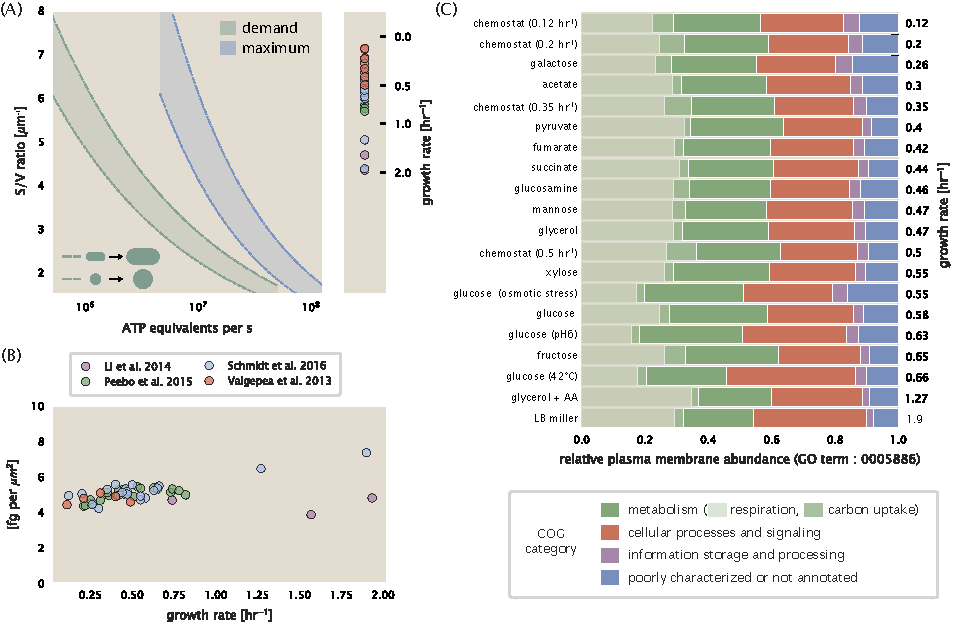
\includegraphics{main_figs/fig5_energy_SV_scaling.pdf}
            \caption{\textbf{Influence of cell size and  S/V ratio on ATP production and inner membrane composition.} (A) Scaling of ATP demand and maximum ATP production as a function of S/V ratio. Cell volumes of 0.5 fl to X fl were considered, with the dash line corresponding to a cell with spherical shape, which the dash-dot line reflects a rod-shaped bacterium like \textit{E. coli} with aspect ratio of 4. (B) Total protein mass calculated for proteins with inner membrane annotation (GO term: 0005886).  (C) Relative protein abundances by mass based on  COG annotation. Metabolic proteins are further separated into respiration (F$_1$-F$_O$ ATP synthase, NADH dehydrogenase I, succinate:quinone oxidoreductase, f cytochrome bo$_3$ ubiquinol oxidase,  cytochrome bd-I ubiquinol oxidase) and carbohydrate transport (GO term: GO:0008643). Note that the elongation factor EF-Tu can also be associated with the inner membrane, but were excluded in this analysis due to their high relative abundance.}
        \label{fig:energy_scaling}
        }
    \end{fullwidth}
\end{figure}
